%TODO: comment on cost of thinning as inductive values?
%      cite the preprint solving this & whose diagram this is?
\newcommand{\cseexamplegraph}{
\begin{tikzpicture}
% \draw (0,0)      node[draw,dashed,regular polygon, regular polygon sides=3, shape border rotate=270]{$E[\cdot]$};
\draw (1.6,0)    node[draw,diamond,align=center] {\$};

\draw (3.75,.75) node[draw, diamond,align=center] {$\lambda x.$};
\draw (6.90,.75) node[draw,dashed,regular polygon, regular polygon sides=3, shape border rotate=90]
      {\phantom{b}$t$\phantom{g}};

\draw (3.75,-.75) node[draw, diamond,align=center] {$\lambda a.$};
\draw (5.90,-.75) node[draw, diamond,align=center] {$\lambda b.$};
\draw (9.05,-.75) node[draw,dashed,regular polygon, regular polygon sides=3, shape border rotate=90]
      {\phantom{b}$t$\phantom{g}};

\draw [->] (1.83,.23)  to [out=45,in=180] (3.2,.75);
\draw [->] (1.83,-.23) to [out=-45,in=180] (3.2,-.75);

\draw [->] (4.35,-.75) to [out=0,in=180]  (5.35,-.75);
\draw [->] (4.35,.75)  to [out=0,in=180]  (5.9,.75);

\draw [->] (6.5,-.75) to [out=0,in=180]  (8,-.75);

% \draw [->] (.23,-.23) to [out=-45,in=180]
\end{tikzpicture}}

\newcommand{\codebruijnexamplegraph}{
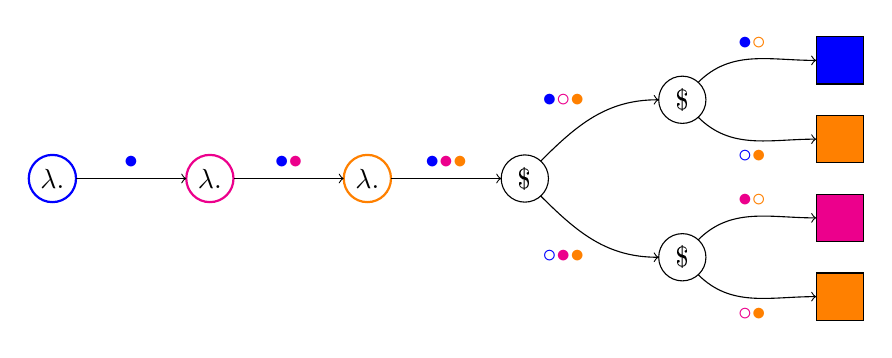
\begin{tikzpicture}
\draw[draw=blue   ,thick] (0,0) circle (.3cm) node[align=center] {$\lambda{}.$};
\draw[draw=magenta,thick] (2,0) circle (.3cm) node[align=center] {$\lambda{}.$};
\draw[draw=orange ,thick] (4,0) circle (.3cm) node[align=center] {$\lambda{}.$};

\draw (6,0) circle (.3cm) node[align=center] {\$};

\draw (8,1)    circle (.3cm) node[align=center] {\$};
\draw[fill=blue]   (10,1.5) +(-.3cm,-.3cm) rectangle +(.3cm,.3cm);
\draw[fill=orange] (10,.5)  +(-.3cm,-.3cm) rectangle +(.3cm,.3cm);

\draw (8,-1)    circle (.3cm) node[align=center] {\$};
\draw[fill=magenta] (10,-.5)  +(-.3cm,-.3cm) rectangle +(.3cm,.3cm);
\draw[fill=orange]  (10,-1.5) +(-.3cm,-.3cm) rectangle +(.3cm,.3cm);


\draw [->] (0.3,0)   to [out=0,in=180] node[above]{$\color{blue}{\bullet}$} (1.7,0);
\draw [->] (2.3,0)   to [out=0,in=180] node[above]{$\color{blue}{\bullet}\color{magenta}{\bullet}$} (3.7,0);
\draw [->] (4.3,0)   to [out=0,in=180] node[above]{$\color{blue}{\bullet}\color{magenta}{\bullet}\color{orange}{\bullet}$} (5.7,0);

\draw [->] (6.2,-.22)  to [out=-45,in=180] node[below left]{$\color{blue}{\circ}\color{magenta}{\bullet}\color{orange}{\bullet}$} (7.7,-1);
\draw [->] (6.2,.22)   to [out=45,in=180] node[above left]{$\color{blue}{\bullet}\color{magenta}{\circ}\color{orange}{\bullet}$} (7.7,1);
\draw [->] (8.2,1.22)  to [out=45,in=180] node[above]{$\color{blue}{\bullet}\color{orange}{\circ}$} (9.7,1.5);
\draw [->] (8.2,.78)   to [out=-45,in=180] node[below]{$\color{blue}{\circ}\color{orange}{\bullet}$} (9.7,.5);
\draw [->] (8.2,-.78)  to [out=45,in=180] node[above]{$\color{magenta}{\bullet}\color{orange}{\circ}$} (9.7,-.5);
\draw [->] (8.2,-1.22) to [out=-45,in=180] node[below]{$\color{magenta}{\circ}\color{orange}{\bullet}$} (9.7,-1.5);
\end{tikzpicture}
}


Now that our core language is well scoped by construction, our compiler passes
must also be shown to be scope-preserving.
%
This is not a new requirement, merely it makes concrete a constraint that
used to be enforced informally.
More importantly we show, with our compiler passes, that model-to-same-model transformation of our \ac{edsl} is possible, and that the infrastructure required is not bespoke to \Velo{}.

The purpose of \ac{cse} is to identify subterms that appear multiple times in the syntax tree, and to abstract over them to avoid needless recomputations at runtime.
%
In the following example for instance, we would like to let-bind $t$ before
the application node (denoted \$) so that $t$ may be shared by both subtrees.

\begin{center}
  \cseexamplegraph{}
\end{center}

One of the challenges of \ac{cse}, as exemplified above, is that the term of interest
may be burried deep inside separate contexts.
%
In our intrinsically scoped representation, $t$ in scope $\Gamma, x : \sigma$ is potentially not actually syntactically equal to a copy living in $\Gamma, a : \tau, b : \nu$.
%
Indeed a variable $v$ bound in $\Gamma$ will, for instance, be represented by
the \DeBruijn{} index $1+v$ in $\Gamma, x : \sigma$
but by the index $2+v$ in $\Gamma, a :  \tau, b : \nu$.

If only terms were indexed by their exact \emph{support}!
We would not care about additional yet irrelevant variables that happen to be in scope.
%
The principled solution here is to switch to a different representation for
the purpose of \ac{cse}.
The co-\DeBruijn{} representation~\cite{DBLP:journals/corr/abs-1807-04085} provides exactly this guarantee.

%\subsection{Co-De Bruijn representation}

In the co-\DeBruijn{} representation, every term is precisely indexed by its
exact support.
%
That is to say that every subterm explicitly throws away the bound variables
that are not mentioned in it.
%
By the time we reach a variable node, a single bound variable remains in scope:
precisely the one being referred to.

If we think of thinnings as sequences of 0/1 bits stating whether a variable
is kept or dropped, and admitting that such sequences can be represented as
list of either $\bullet$ (1) or $\circ$ (0), the $S$ combinator
($\lambda g. \lambda f. \lambda x. g x (f x)$) is represented as follows in
co-\DeBruijn{} notation.

\begin{center}
  \codebruijnexamplegraph{}
\end{center}

The first three $\lambda$ abstractions only use $\bullet$ in their thinnings
because all of $g$, $f$, and $x$ do appear in the body of the combinator.
%
The application node then splits the context into two: the first subterm
($g x$) drops $f$ while the second ($f x$) gets rid of $g$.
%
Further application nodes select the one variable still in scope for each
leaf subterm: $g$, $x$, $f$, and $x$.


Using a co-\DeBruijn{} representation, we can easily identify shared subterms:
they need to not be mentioning any of the most local variables and be
syntactically equal.
